\subsection{Consistency checks of the model}
\label{app:MC}


In this appendix we perform several checks of our model.
At first, we investigate the relative importance of prior and covariate shifts by comparing models with only prior or only covariate shift to the full model that contains both prior and covariate shifts. 
%(cf \ref{}). 
We then proceed to perform consistency checks. We start by generating distributions of sources in parameter space from our best-fit model (including only astrophysical components) and fit the generated data with the same model.
%(cf. \ref{}). 
The goal is to determine a distribution of $\log\mathcal{L}$ values due to statistical fluctuations (since the data was generated from this model) and to compare to the value of $\log\mathcal{L}$ for the actual data to check if the model without a DM contribution is generally a good fit to the data.
As a last consistency check, we perform injection tests, where we add a DM subhalo component to the astro-only model to check if we can recover the injected signal.
%(cf \ref{}).

\subsection{Importance of covariate and prior shifts}
\label{app:prior_vs_cov}

In order to investigate the importance of the prior and covariate shifts, 
we first compare the performance of four models in eq. (\ref{eq:mixture}) without the DM component: a model without either prior or covariate shifts (i.e., no free parameters) determined from associated sources, denoted as ``$as$'', models with only prior or covariate shifts, denoted as ``$p$'' or ``$c$'' respectively, and a model with both prior and covariate shifts, denoted as ``$p+c$''. 

The model without either prior or covariate shifts is constructed from the catalog of associated sources following sections \ref{sec:cov_prior} and \ref{sec:stat-model}, where the prior probability of a class is given by the relative class prevalence $\pi_k$ in the 4FGL-DR4 catalog, while the PDFs of the Galactic and extragalactic components are derived from the corresponding associated sources.
The model with either prior or covariate shift follows eq. (\ref{eq:mixture}), 
where we fix the covariate shift modulation to be equal to 1 (i.e., $\tilde{C}(\bx; \btheta_\textrm{cov}) = 1$), or fix the prior probabilities to the corresponding values for associated sources.


% table to compare models
\begin{table*}[t]
\centering
\resizebox{0.95\textwidth}{!}{
\begin{tabular}{|lcccc|ccc|}
\toprule
model & $2\Delta \log \LL_{as,x}$ & $\Delta\textrm{dof}_{as,x}$ & $N\sigma_{as,x}$ & $\textrm{AIC}_{as,x}$ & $2\Delta \log \LL_{x,p+c}$ & $\Delta\textrm{dof}_{x,p+c}$ & $N\sigma_{x,p+c}$\\
\midrule
associated          & 0       & 0  & 0.0  & -178 &  64.7 & 7 & 6.7\\
prior               & 49.5    & 1  & 7.0  & -225 & 14.2 & 6 & 2.2\\
covariate           & 33.4    & 6  & 4.5  & -199 & 30.3 & 1 & 5.5 \\
prior + covariate   & 64.7    & 7  & 6.7  & {-227} & 0.0  & 0 & 0.0 \\
\bottomrule
\end{tabular}
}
\caption{Comparison of models of unassociated sources with Galactic and extragalactic components. ``as'' denotes the model derived from distributions of associated sources applied to the unassociated sources (without free parameters). ``$p+c$'' is the full covariate + prior shift model. 
Subscipt ``$x$'' denotes the model specified in the first column of the table.
For example, the value of $2\Delta \log \LL_{as,x} = 33.4$ in the fourth row and second column corresponds to the difference between the model derived for associated sources and the model with only covariate shift, i.e., to $x = c$ (covariate) in this case.
}
\label{tab:models}
\end{table*}


We compare the performance of the four models evaluated on the unassociated sources in the ROI for $E_0$ = 1 GeV in table \ref{tab:models}.
In column 2, we show the difference in log likelihood between the model specified in the first column and the model based on distributions of associated sources.
We report the corresponding additional degrees of freedom in column 3.
We find that the prior shift model leads to a larger increase in likelihood for one degree of freedom (we have a constraint that the sum of priors is equal to 1: $\pi_\textrm{gal} + \pi_\textrm{ext} =1$) compared to a model with covariate shift only.
The corresponding significance of exclusion of the null hypothesis (the ``as'' model) is presented in column 4.
It is derived by assuming the $\chi^2$ distribution for $-2\Delta \log \mathcal{L}$ with the corresponding number of degrees of freedom from column 3.
In column 5 we show the Akaike information criterion, $\textrm{AIC} = -2\log\mathcal{L} + 2 k$, where $k$ is the number of degrees of freedom.
We find that although log likelihood of the full prior $+$ covariate shift model is the largest,
both the significance of exclusion of the null hypothesis and the AIC for this model are comparable to the ones for the prior shift only model.
Thus, we conclude that the prior shift is the dominant effect compared to the covariate shift.
We further compare the models in column 1 to the full prior $+$ covariate shift model in columns 6, 7, and 8, where we show $2\Delta \log \mathcal{L}$, the additional degrees of freedom, and the significance of exclusion of the null hypothesis, which, in this case, is the model in the first column.
In particular, we find that the prior shift model can be excluded only at 2.2 sigma level in favor of the ``$p + c$'' model.


In figure~\ref{fig:1d-marginals},
we compare our models with the distributions of parameters $\alpha$, $\beta$, and $\log_{10}(\phi)$ for the unassociated sources. 
We display the best-fit ``$p+c$'' model (in red) and compare it with the prior KDE model derived for associated sources (in blue).
The ``$p+c$'' model provides a reasonable fit to the data for all the distribution parameters. On the other hand, the model derived for associated sources fails to capture the $\beta$ dependence correctly, as expected, since the distribution for unassociated sources differs considerably from the distribution of associated sources for the $\beta$ parameter (cf. figure~\ref{fig:alpha_beta_hist_E01000MeV}). 


\begin{figure}[t]
    \centering
    \resizebox{0.95\textwidth}{!}{
    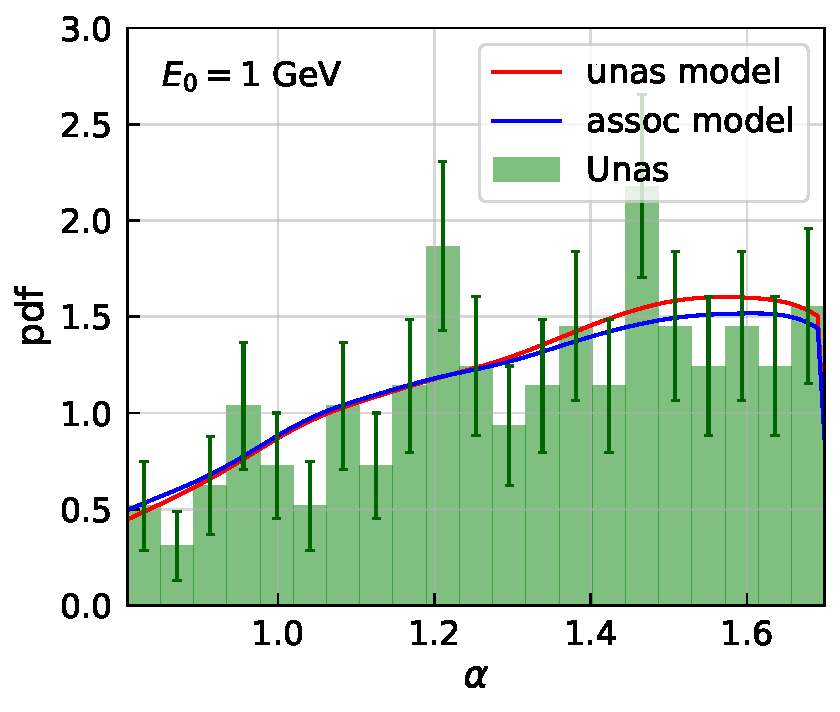
\includegraphics[width=0.30\linewidth]{sections/paper_dm_halos/img/model0/marginal_alpha_30GeV.pdf}
    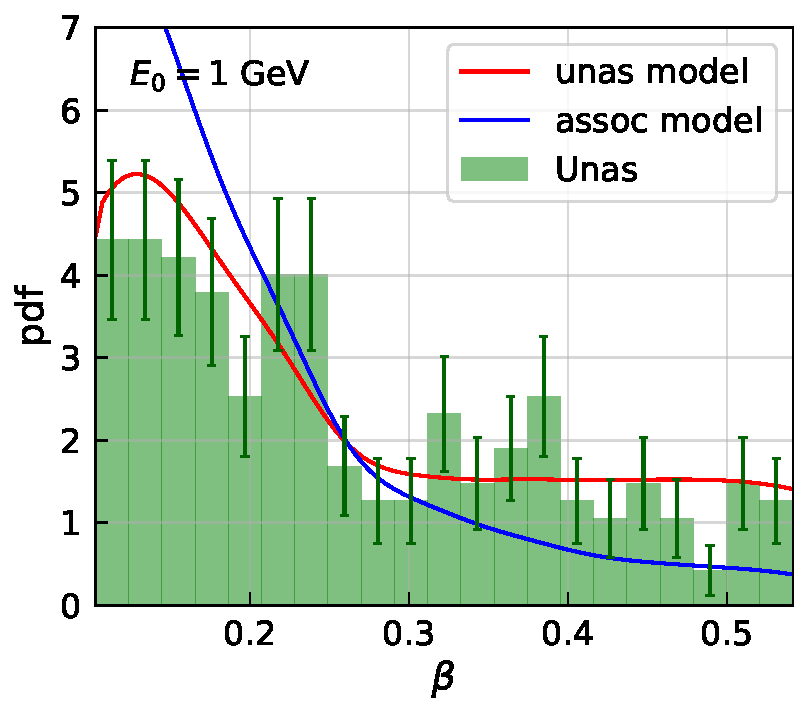
\includegraphics[width=0.30\linewidth]{sections/paper_dm_halos/img/model0/marginal_beta_30GeV.pdf}
    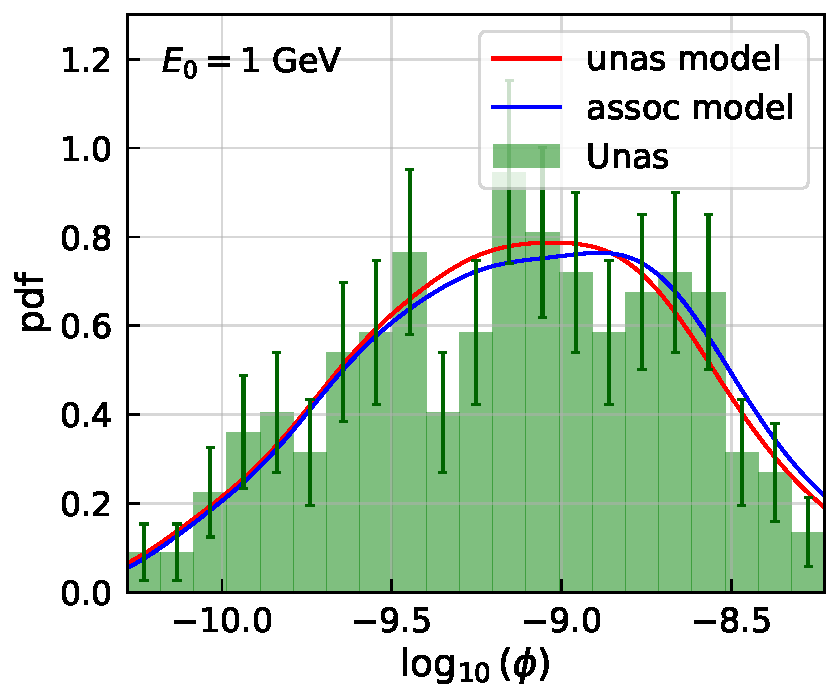
\includegraphics[width=0.30\linewidth]{sections/paper_dm_halos/img/model0/marginal_log10phi_30GeV.pdf}
    }
    \caption{Distributions of the $\alpha$, $\beta$ and $\log_{10}(\phi)$ parameters 
    for the unassociated sources in the 4FGL-DR4 catalog. 
    The bars show statistical uncertainty.
    The best-fit model that includes both covariate and prior shifts is shown by the red line while the model derived for associated sources is shown by the blue line. The 3D model is integrated in two variables to obtain the distribution in the third variable, shown on the plot.
    }
    \label{fig:1d-marginals}
\end{figure}

\subsection{Bootstrap MC and overall goodness of fit}
\label{app:model_goodness}

\begin{figure}[t]
    \centering
    \resizebox{0.95\textwidth}{!}{
    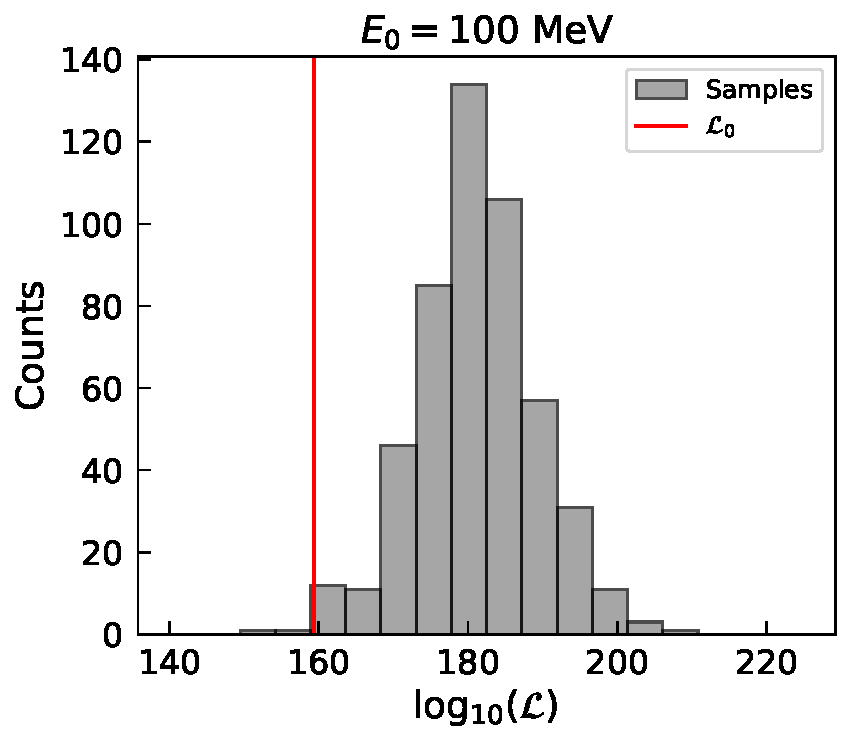
\includegraphics[width=0.45\linewidth]{sections/paper_dm_halos/img/model0/likelihood_samples_model0_covariate_shift_E0_100.pdf}
    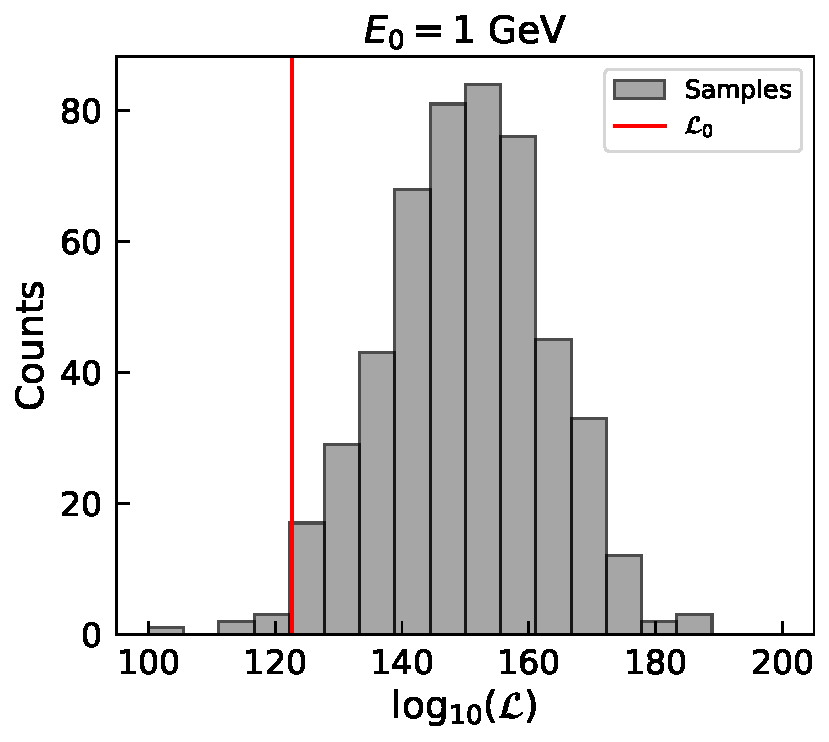
\includegraphics[width=0.45\linewidth]{sections/paper_dm_halos/img/model0/likelihood_samples_model0_covariate_shift_E0_1000.pdf}
    }
    \caption{Distribution of log-likelihood for the ``$p+c$'' model with astro-only components for 1000 datasets simulated from the best-fit ``$p+c$'' model for $E_0=100 \, \textrm{MeV}$ (\panel{left panel}) and $E_0=1 \, \textrm{GeV}$ (\panel{right panel}). The red line represents the log-likelihood of the ``$p+c$'' model with astro-only components for the unassociated 4FGL-DR4 sources.}
    \label{fig:loglike-bootstrap}
\end{figure}

We quantitatively estimate the goodness of fit of the ``$p + c$'' model in figure~\ref{fig:loglike-bootstrap}.
In this figure, we generate samples of sources in the parameter space from the best-fit ``$p + c$'' model. We then reoptimize the model for each of the samples.
The corresponding distribution of the log likelihood values has only statistical fluctuations.
The red lines on these plots show the best-fit $\log \mathcal{L}$ value for the real data.
These values are about 2 sigma smaller than the mean of the $\log \mathcal{L}$ distribution both for $E_0 = 100$~MeV (left panel) and for $E_0 = 1$~GeV (right panel).
On the one hand, this deviation shows that the model is not perfect, i.e., there are possibly some deviations of the model and the data.
On the other hand, the deviation has only about 2 sigma statistical significance.
This deviation may be connected to the slight excess observed, e.g., in the $\mdm = 30$~GeV DM annihilation (cf. the $\mdm = 30$~GeV row in Table~\ref{tab:Nsub_values}).
\new{Indeed, if there is an excess at about $2\sigma$ significance, which is not accounted by the model, then the model would be excluded at $2 \sigma$ significance compared to a model that can explain the data without excesses, e.g., the data generated from the model itself (cf. figure~\ref{fig:loglike-bootstrap}).}


% signal injection
\subsection{DM subhalo injection test}
\label{app:DM_injection}

In order to ensure our model is actually capable of reconstructing a DM signal, we inject a DM signal into simulated data and test the ability of our model to reconstruct it.
We choose a significant value of $\sigmav$ for each DM mass. For $\mdm$ = 30, 100, 300 GeV, we adopt the best fit $\sigmav$ value from table \ref{tab:Nsub_values}, while for $\mdm = 10, 1000$ GeV, since the best-fit value is zero, we inject a signal with a $\sigmav$ corresponding to the 3$\sigma$ significance (which should be clearly distinguishable from the null hypothesis). 

\begin{figure}[t]
    \centering
    
    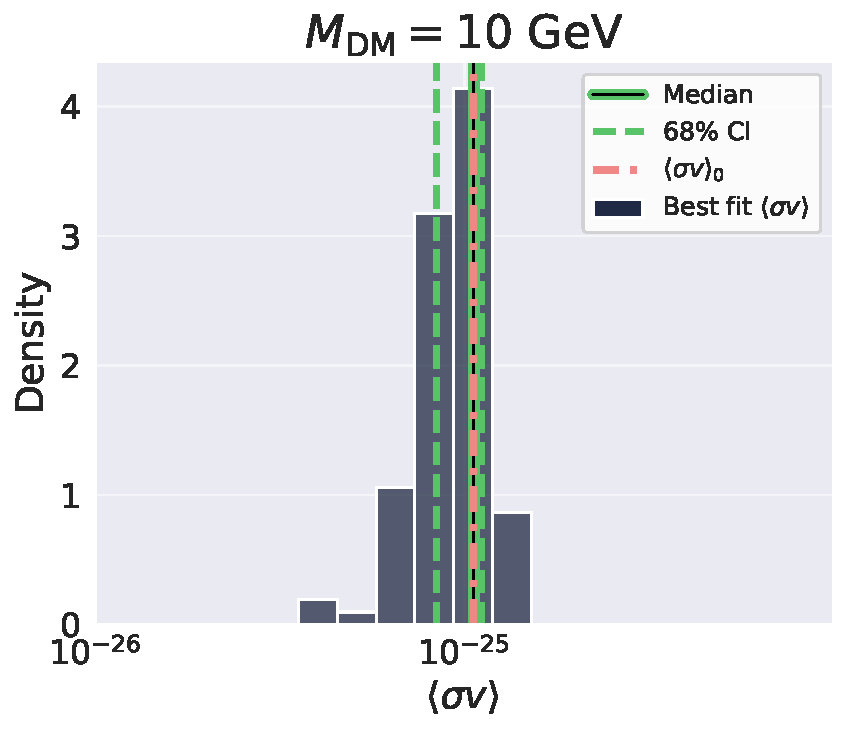
\includegraphics[width=0.45\linewidth]{sections/paper_dm_halos/img/signal_injection/signal_injection_mDM_10GeV_v2.pdf}
    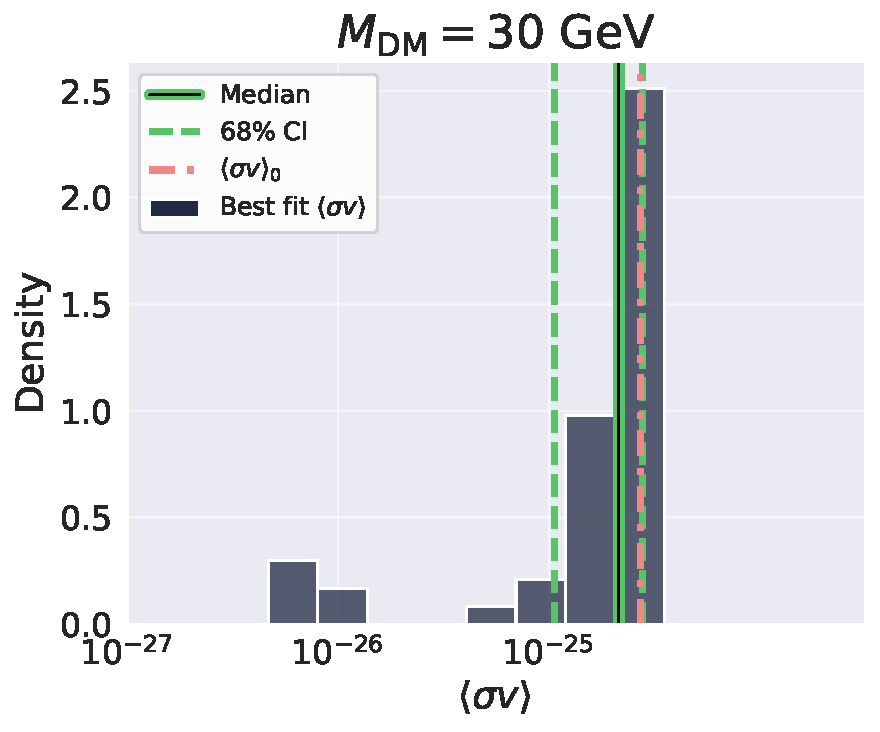
\includegraphics[width=0.45\linewidth]{sections/paper_dm_halos/img/signal_injection/signal_injection_mDM_30GeV_v2.pdf}
    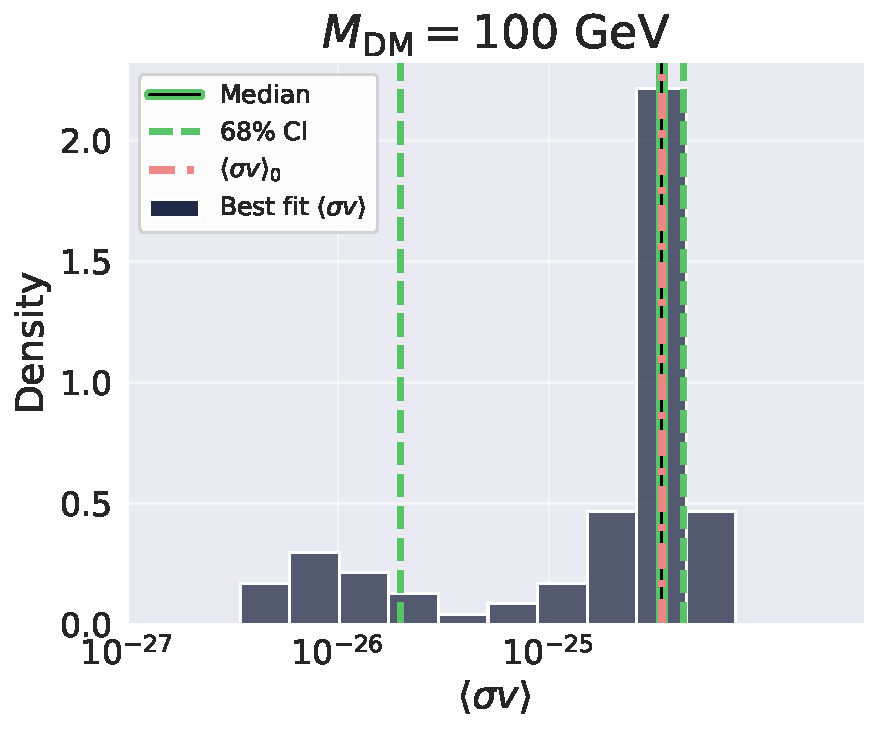
\includegraphics[width=0.45\linewidth]{sections/paper_dm_halos/img/signal_injection/signal_injection_mDM_100GeV_v2.pdf}
    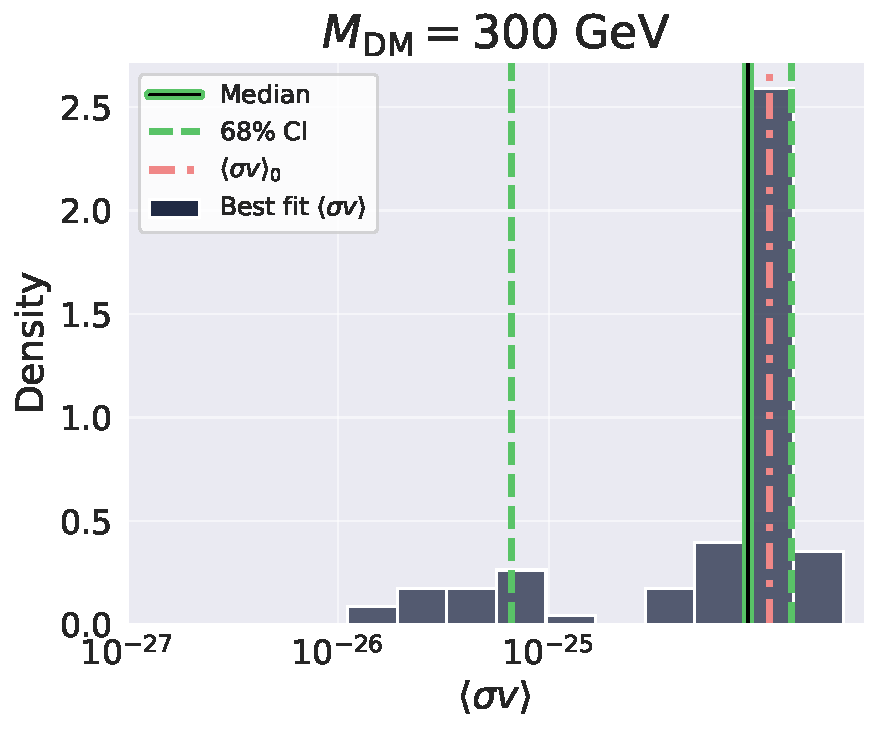
\includegraphics[width=0.45\linewidth]{sections/paper_dm_halos/img/signal_injection/signal_injection_mDM_300GeV_v2.pdf}
    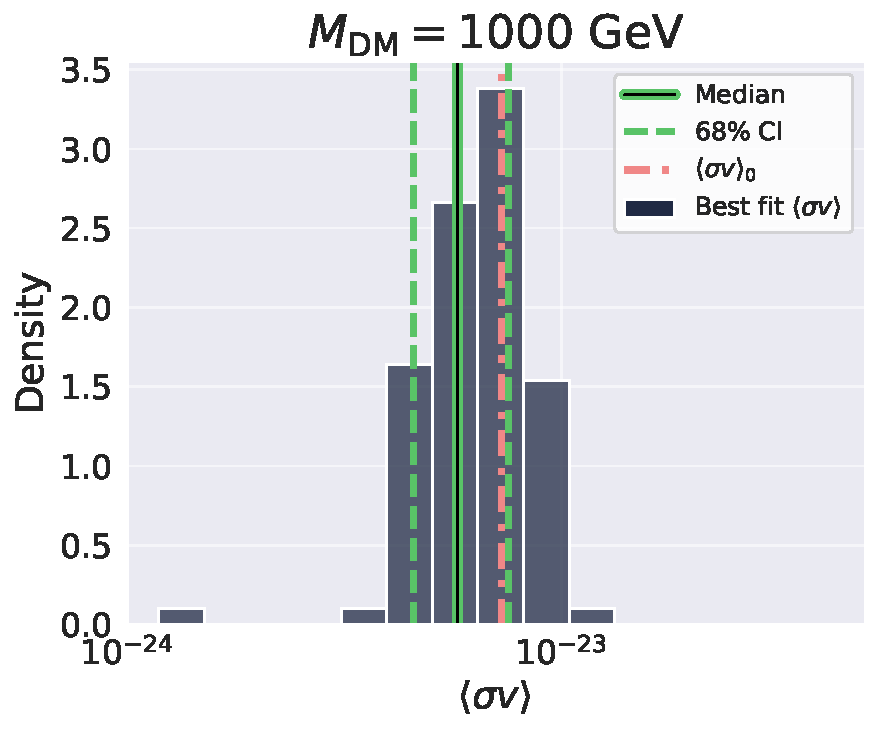
\includegraphics[width=0.45\linewidth]{sections/paper_dm_halos/img/signal_injection/signal_injection_mDM_1000GeV_v2.pdf}

    \caption{
    Histograms representing the reconstructed $\sigmav$ values for simulations with injected DM signals. The red dash-dotted line represents the annihilation cross-section of the injected signal ($\sigmav_0)$. The green solid line represents the median of the distribution, while the green dashed lines show the 68\% containment interval. In every case, the true $\sigmav$ value lies inside the 68\% containment region.
    }
    \label{fig:line-injection}
\end{figure}

We show the histogram of the recovered $\sigmav$ values for the 5 DM masses in figure~\ref{fig:line-injection}.
The $\sigmav$ values for the injected DM signal (red dashed-dotted lines, $\sigmav_0$) are within the 68\% containment interval (green dashed lines) of the histogram
relative to the median values for the distributions (solid green lines).
Thus, our methodology is capable of reconstructing a simulated signal, when present, in the majority of cases. 

Finally, we \old{showcase} \new{illustrate} the model's predictive capabilities. Using eq.~(\ref{gamma}), we derive the posterior probability that each unassociated source belongs to a given class $k$ (e.g., extragalactic, Galactic, or DM). The predicted class label, $C_i^{\text{pred}}$, is then assigned to the class with the highest posterior probability: $C_i^{\text{pred}} = \operatorname{argmax}_k \{ \tilde{p}(z_{ik}=1|\textbf{x}_i) \}$.
Figure~\ref{fig:predictions-real} displays the posterior probabilities and predicted classes for all unassociated sources. The left panel shows results from our best-fit model with only astrophysical classes (for $\textrm{E}_0 = 1 \, \textrm{GeV}$), while the right panel shows the best-fit model including DM (for the $\mdm=30$ GeV case).

\old{To further assess performance,}
\new{For comparison,}
we repeat this exercise on a simulated bootstrap sample for the $\mdm=30$ GeV case in figure~\ref{fig:predictions-bootstrap}. 
The figure compares the true class labels (left panel) with the posterior class probabilities (middle panel) and the final predicted class labels (right panel) for a model fit to the bootstrap sample.
\old{Access to both true labels and posterior probabilities enables a deeper analysis of the model's performance. }
For instance, while not all DM sources were correctly classified due to significant parameter overlap with the Galactic source population, their true class often received a high posterior probability, even if it was not the maximum. This \old{highlights} \new{shows} that to avoid false negatives when identifying a subdominant class, it is \old{crucial} \new{important} to consider \old{all} sources with a \new{reasonably} high posterior probability for that class \new{even if this probability is not the highest}. \old{, not only those where it is the highest.}




\begin{figure}[t]
    \centering
    \resizebox{0.95\textwidth}{!}{
    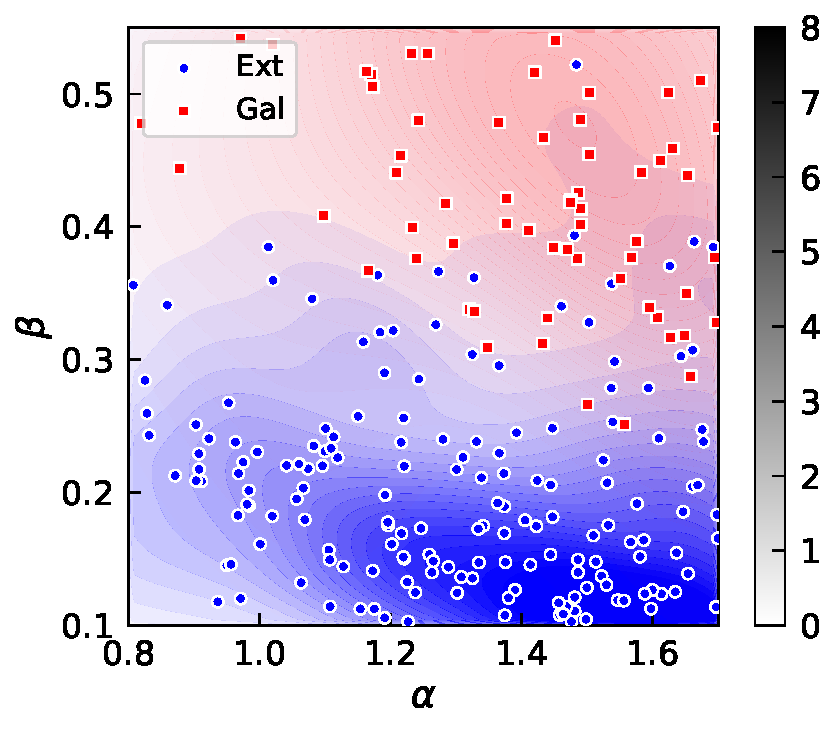
\includegraphics[width=0.45\linewidth]{sections/paper_dm_halos/img/predictions/model0_30GeV_predictions.pdf}
    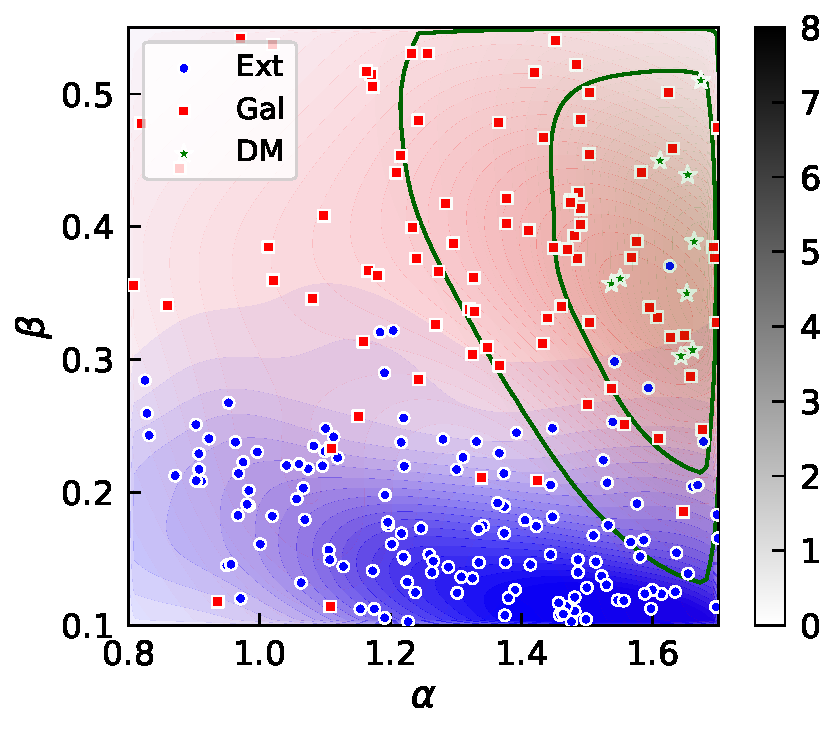
\includegraphics[width=0.45\linewidth]{sections/paper_dm_halos/img/predictions/model_30GeV_predictions.pdf}
    }
    \caption{Predicted source classes for unassociated 4FGL-DR4 sources according to the posterior class probabilities for the $E_0 = 1 \, \textrm{GeV}$ case.
    \panel{Left panel}: best-fit model with astrophysical only classes.
    \panel{Right panel}: best-fit model for astrophysical classes and DM ($\mdm = 30$ GeV, $\sigmav \sim 2.7\cdot 10^{-25} \, \textrm{cm}^{3}\,\textrm{s}^{-1}$). The green contours represent the 68\% and 95\% containment levels for the DM distribution. 
    }
    \label{fig:predictions-real}
\end{figure}

\begin{figure}[t]
    \centering
    \resizebox{0.99\textwidth}{!}{
    \hspace{-3mm}
    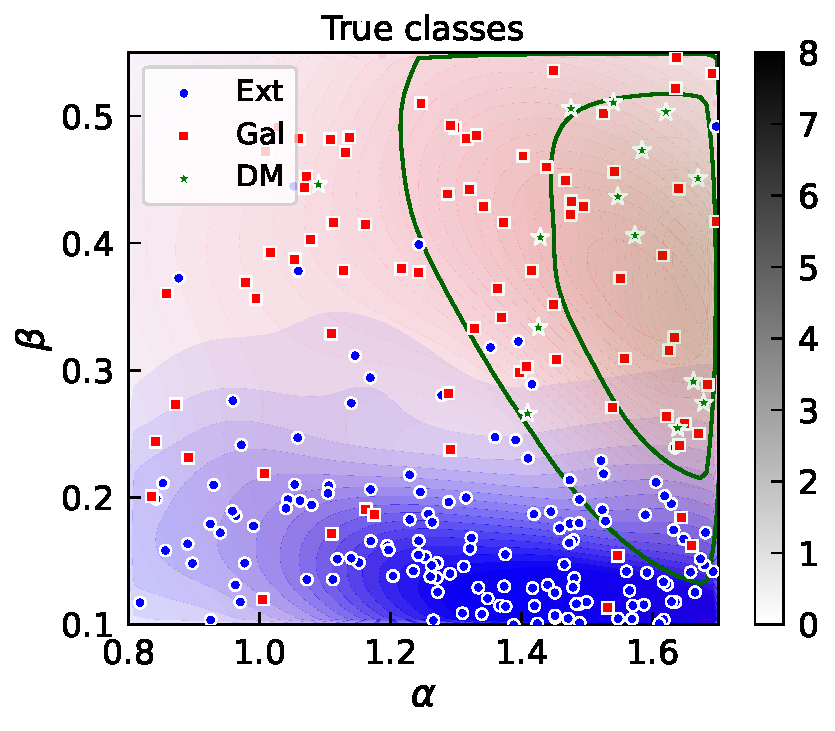
\includegraphics[width=0.33\linewidth]{sections/paper_dm_halos/img/predictions/bootstrap_model_30GeV_true_labels.pdf}
    \hspace{-3mm}
    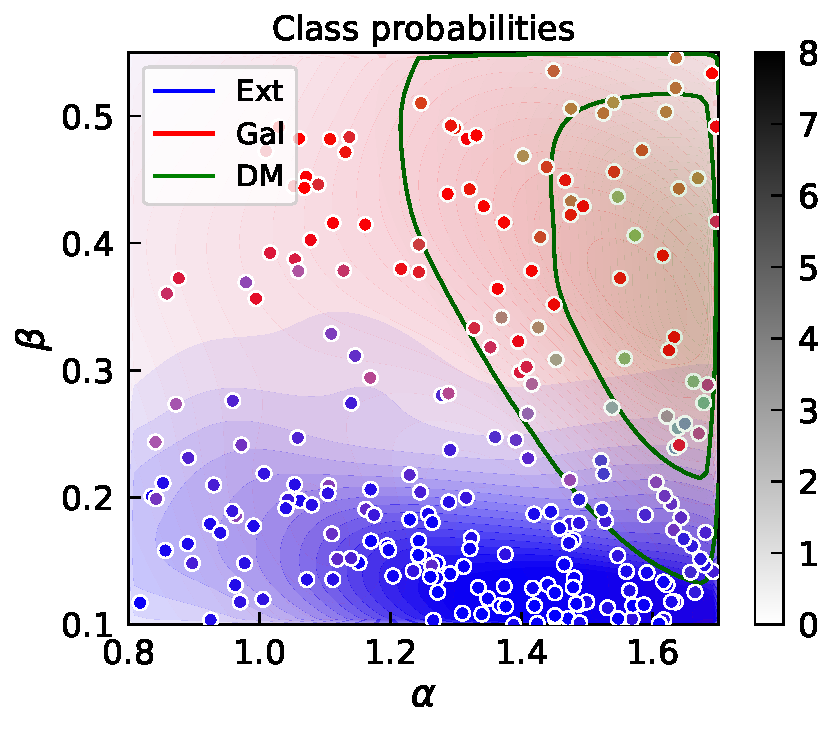
\includegraphics[width=0.33\linewidth]{sections/paper_dm_halos/img/predictions/bootstrap_model_30GeV_posterior_prob_v4b.pdf}
    \hspace{-3mm}
    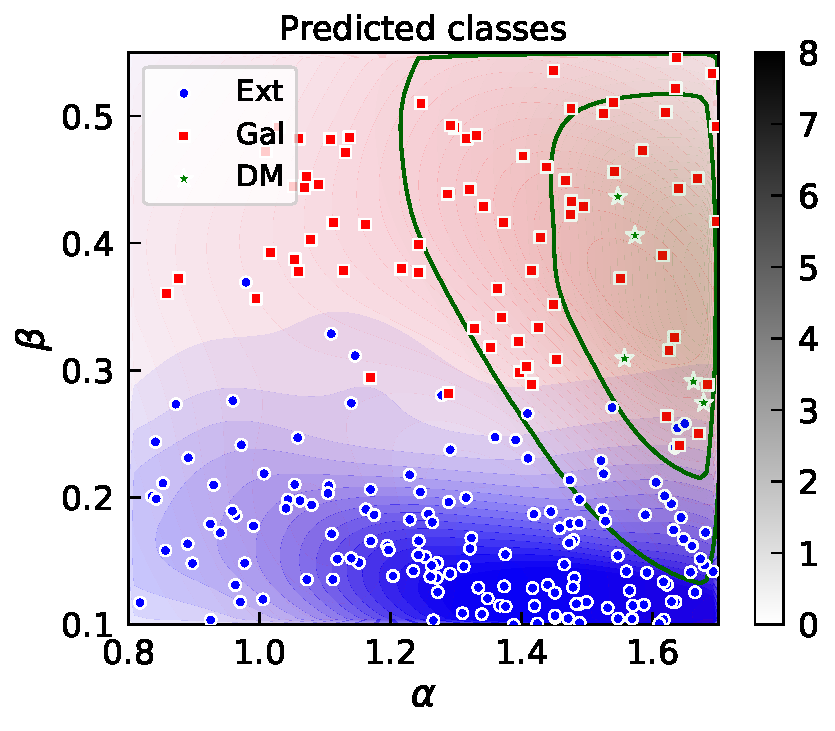
\includegraphics[width=0.33\linewidth]{sections/paper_dm_halos/img/predictions/bootstrap_model_30GeV_predictions.pdf}
    }
    \caption{Estimated best-fit distributions and true or predicted source classes for a bootstrap simulation, with $\mdm = 30$ GeV and $\sigmav \sim 2.7\times 10^{-25} \, \textrm{cm}^{3}\,\textrm{s}^{-1}$.
    \panel{Left panel}: markers colored according to their true class $C_i^{true}$ in the simulation.
    \panel{Middle panel}: markers colored according to their posterior class probability 
    following the same convention as figure~\ref{fig:mixture_DM_tot}.
    \panel{Right panel}: markers colored according to the predicted class, given by $C_i^{pred} = \textrm{argmax}_k \{ \tilde{p}(z_{ik}=1|\textbf{x}_i) \}$.
    }
    \label{fig:predictions-bootstrap}
\end{figure}

\subsection{\new{Precision-recall curves for classification of individual DM subhalos}}
\label{app:pr_curve}

\new{
To further quantify the model's ability to distinguish DM subhalos from the astrophysical background, we perform a Precision-Recall (PR) analysis for the case of $\mdm = 30$~GeV.
This DM mass yields the highest 
possible signal due to DM annihilation in subhalos (cf. table~\ref{tab:Nsub_values})
but it is also
challenging due to the extensive spectral overlap with Galactic sources. 
The PR framework is more relevant here than the Receiver Operating Characteristic curves for highly unbalanced datasets, as it focuses exclusively on the minority class (the signal), providing a rigorous assessment of how many ``DM-like" candidates are likely to be actual subhalos without being skewed by the overwhelming abundance of background sources.
}

\new{
We consider two physical scenarios for the annihilation cross-section: the best-fit value obtained in our primary analysis ($\sigmav = 2.7 \times 10^{-25} \text{ cm}^3/\text{s}$) and a value close to the 95\% upper bound ($\sigmav = 3.6 \times 10^{-25} \text{ cm}^3/\text{s}$). For each scenario, we evaluate the PR performance across a suite of 1000 independent simulations.
In figure~\ref{fig:pr-curves}, we display the mean PR curve along with the 68.27\% asymmetric confidence band derived from the simulation quantiles, representing the expected statistical variance due to background realizations and Poisson noise.
}
\\
\new{
To quantify performance, we compute the Average Precision (AP):
\be
AP = \sum_n (R_n - R_{n-1}) P_n
\ee
where $P_n$ and $R_n$ are the precision and recall at the $n$-th classification threshold. We find $AP = 0.40 \pm 0.16$ for the best-fit case and $AP = 0.50 \pm 0.14$ for the upper bound. 
These scores significantly outperform their respective random chance baselines of 0.03 and 0.06.
The fact that the AP remains below unity is a direct reflection of the intrinsic physical confusion between DM subhalos annihilating in the $b\bar{b}$ channel for $\mdm = 30$~GeV and Galactic millisecond pulsars.
}

\begin{figure}[t]
    \centering
    \resizebox{0.99\textwidth}{!}{
    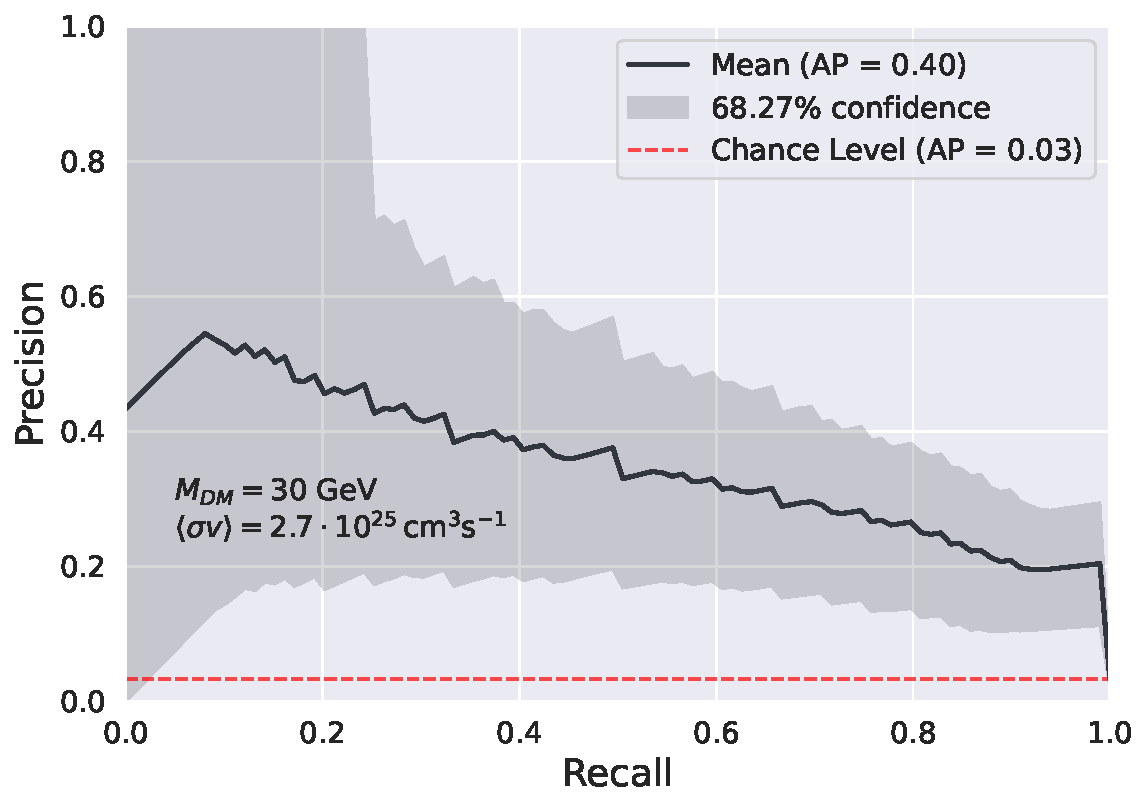
\includegraphics[width=0.49\linewidth]{sections/paper_dm_halos/img/predictions/pr_curve_best_fit.pdf}
    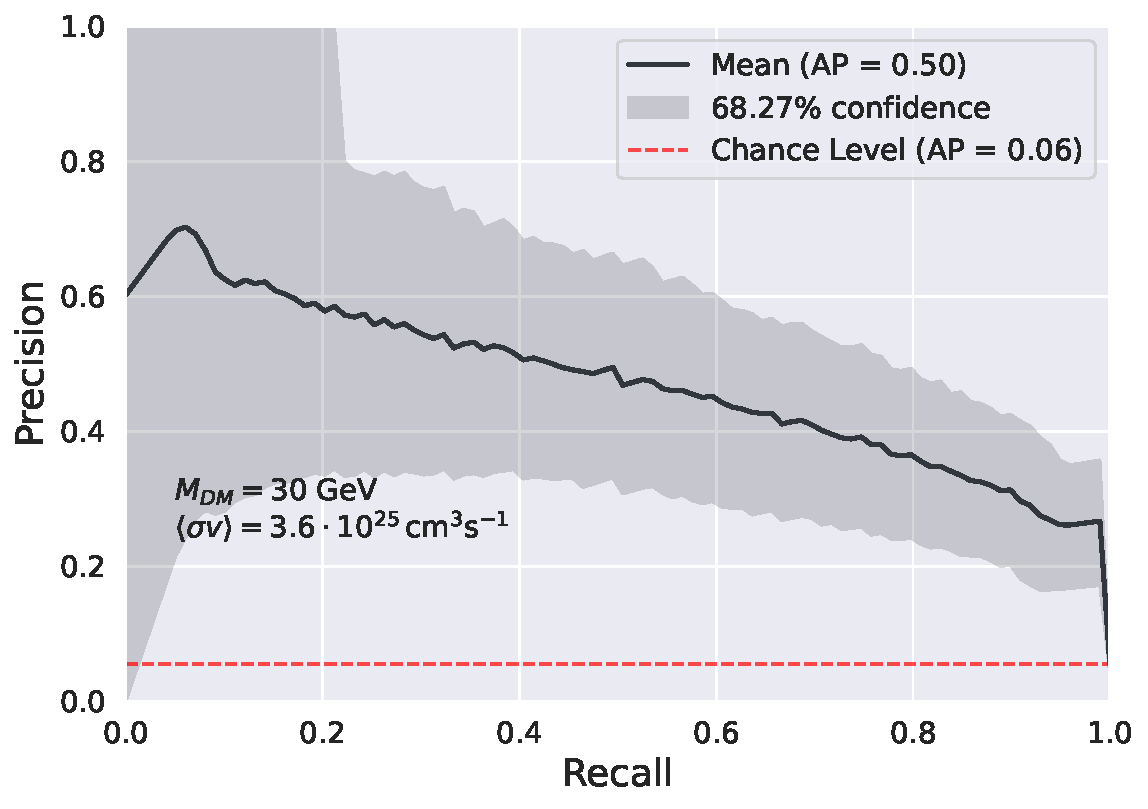
\includegraphics[width=0.49\linewidth]{sections/paper_dm_halos/img/predictions/pr_curve_bound.pdf}
    }
    \caption{
    \new{
    Precision and recall for classification of individual DM subhalos among unassociated \Fermi-LAT sources.
    Solid black line (gray band) shows the mean (68.27\% statistical containment) for 1000 simulations at $\mdm = 30$~GeV. \panel{Left panel}: performance for the best-fit cross-section in table~\ref{tab:Nsub_values} (average precision $AP = 0.40 \pm 0.16$). \panel{Right panel}: performance for a cross-section close to the 95\% confidence upper bound in table~\ref{tab:Nsub_values} ($AP = 0.50 \pm 0.14$).}
    }
    \label{fig:pr-curves}
\end{figure}


%%%%%%% end 

